% pScientists typically have to seek out the aid of software developers in order to obtain configuration files that matched their specifications. This is currently being done manually by editing large JSON files which is both fragile as well as time-consuming for both parties involved.

The NeXus Constructor is a tool written with Qt for Python which allows scientists to create, edit and visualise NeXus files with minimal assistance. Such files can then be used for configuring the experiment control software in order to write real-time data. The layout of the NeXus Constructor interface consists of the following elements:

% Someone may not know what experiment control software does, what makes real-time data good, etc.

\begin{itemize}
\item Instrument View - A Qt3D pane that draws the experiment components in 3D. As NeXus files can contain information about a component's geometry and any transformations that may have been applied to it, translating this into something Qt3D can understand is fairly simple.
\item Component List - A list of the components in the NeXus file.
\item NeXus File Layout - An illustration of the hierarchical NeXus structure. Can't be used to see the values of the individual fields, but can serve as a tool through which you can check that the data has a sensible arrangement. Because the NeXus format is based on HDF5, the \texttt{h5py} library is able to interpret NeXus files so that we may display their layout in our application.
\end{itemize}

To add a component a user presses the "Add Component" button. This causes an additional window to open that allows the user to enter the properties of the component such as its name, its shape, and its description. The application performs some basic checks as this is entered in order to make sure the information is valid. When the user is done 

\begin{figure}
\caption{Screenshot of the NeXus Constructor}
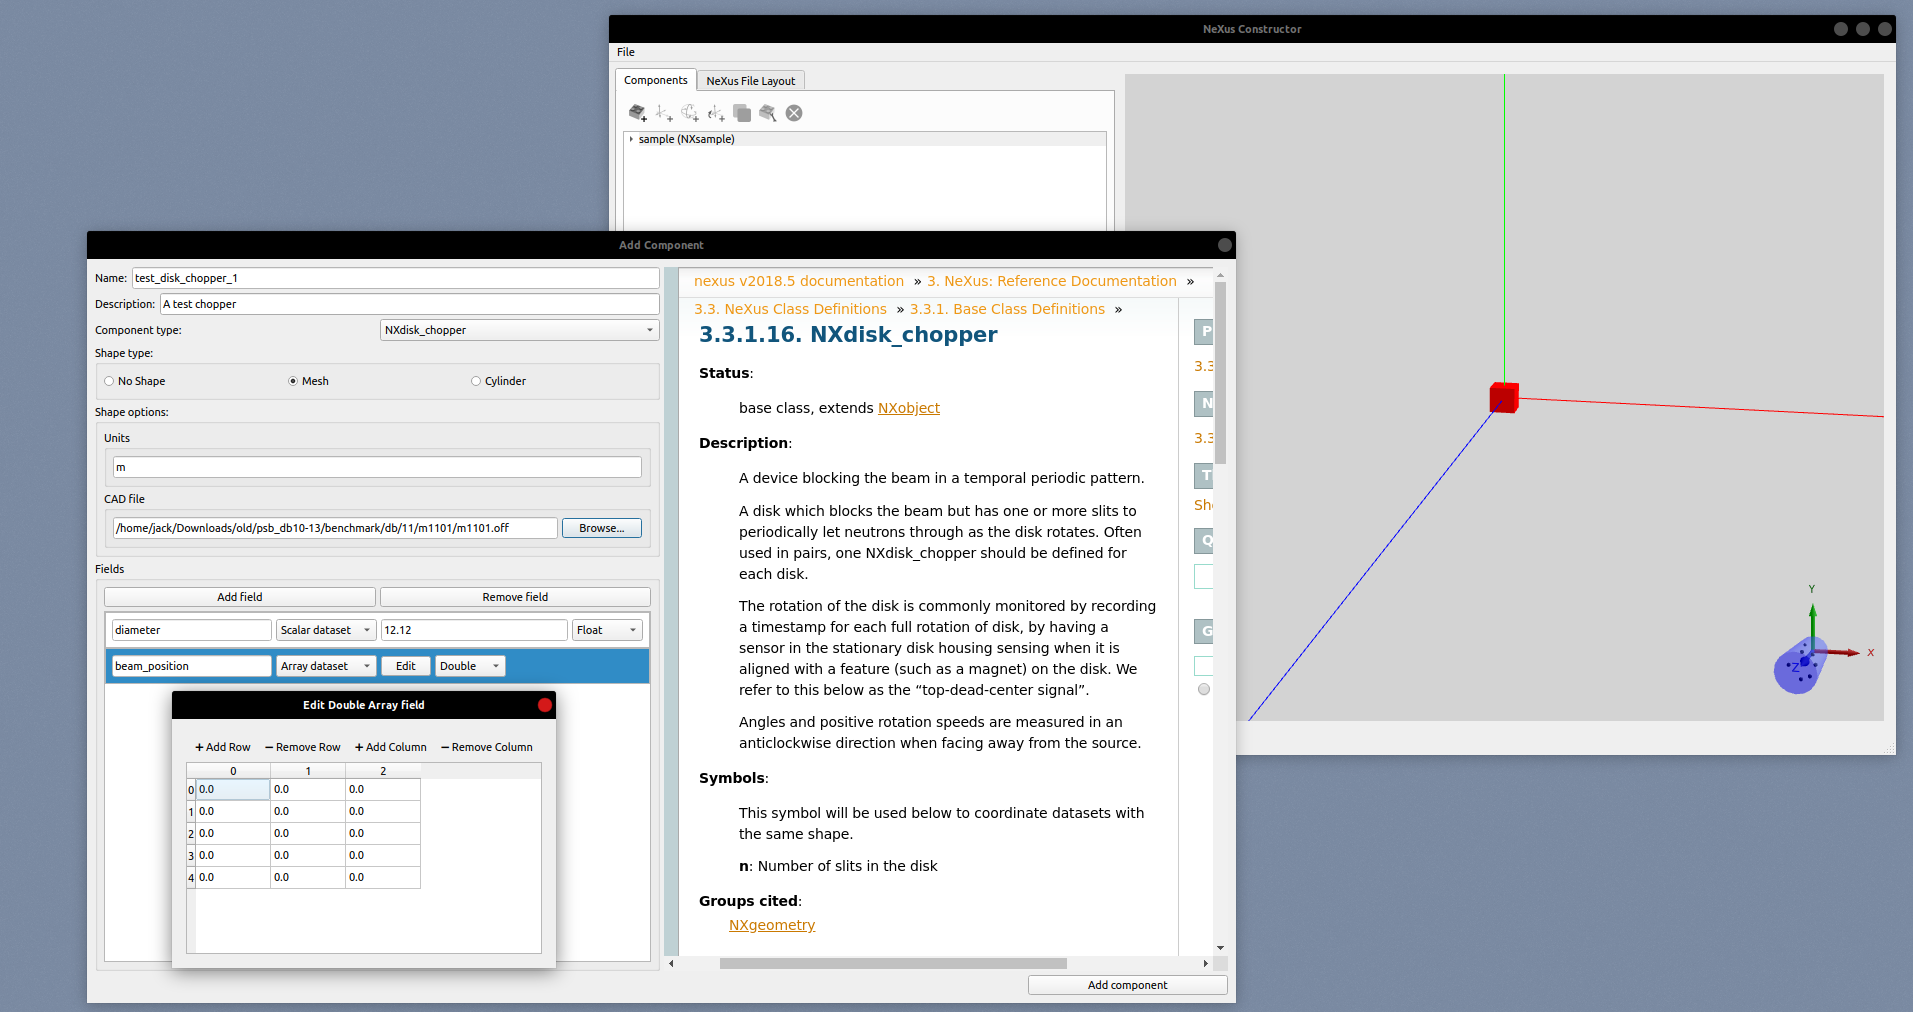
\includegraphics[width=\linewidth]{screenshot.png}
\end{figure}

The screenshot shows the main window of the NeXus Constructor and its "Add Component" dialog which allows users to add extra data in a NeXus file that describes the components that were present in an experiment.




